\documentclass[11pt, a4paper]{article}
\usepackage[utf8]{inputenc}
\usepackage[T1]{fontenc}
\usepackage{helvet}
\renewcommand{\familydefault}{\sfdefault}
\usepackage[table]{xcolor}
\definecolor{schoolgreen}{HTML}{92D050}
\usepackage{geometry}
\geometry{landscape, margin=1.5cm, top=4cm, headheight=2.5cm, headsep=0.5cm}
\usepackage{array}
\usepackage{graphicx}
\usepackage{fancyhdr}
\usepackage{longtable}
\usepackage{amssymb}
\pagestyle{fancy}
\fancyhf{}
\fancyhead[L]{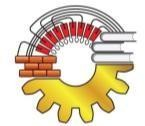
\includegraphics[height=2cm]{../../distritos/4117/templates/logo1.jpg}}
\fancyhead[R]{
\includegraphics[height=2cm]{../../distritos/4117/templates/logo2.jpg}}
\fancyhead[C]{\fontsize{10}{12}\selectfont \textbf{\textit{ESCUELA N.° 4-117 EJÉRCITO DE LOS ANDES \\ DIRECCIÓN DE EDUCACIÓN TÉCNICA Y TRABAJO \\ SECCIÓN V}}}
\renewcommand{\headrulewidth}{0pt}

\begin{document}
\noindent\colorbox{schoolgreen}{\begin{minipage}{\dimexpr\textwidth-2\fboxsep}\centering \textbf{\fontsize{14}{16}\selectfont PLANIFICACIÓN ANUAL 2026}\end{minipage}}

\vspace{1em}
\begin{flushleft}
\textbf{Espacio Curricular:} Prácticas Profesionalizantes \\
\textbf{Ciclo Lectivo:} 2026 \\
\textbf{Curso:} 5to 3ra \\
\textbf{Profesor Responsable:} Ferreyra Gustavo David
\end{flushleft}

\vspace{1em}
\noindent \textbf{FUNDAMENTACIÓN:}
\textit{Las Prácticas Profesionalizantes constituyen el núcleo de la formación técnica, permitiendo que el alumno integre los conocimientos teóricos de diversas materias en situaciones reales de trabajo. El objetivo es desarrollar competencias profesionales que incluyan la capacidad de organizar tareas, aplicar normas de seguridad industrial y resolver problemas técnicos con autonomía y responsabilidad, preparando al estudiante para la inserción laboral o la educación superior.}

\vspace{1em}
\noindent \textbf{ACUERDOS DE ÁREA:}
\begin{itemize}
\item Cumplimiento estricto del uso de Elementos de Protección Personal (EPP).
\item Responsabilidad en el cuidado y mantenimiento del equipamiento del taller.
\item Valoración de la puntualidad y la organización del flujo de trabajo.
\end{itemize}

\vspace{1em}
\noindent \textbf{CAPACIDADES INSTITUCIONALES:}
\begin{itemize}
\item Comprender y producir textos orales y escritos con eficacia y autonomía.
\item Aplicar conocimientos, habilidades, destrezas, actitudes y valores en la resolución y planteo de situaciones problemáticas con creatividad, eficacia, eficiencia, calidad, seguridad y productividad.
\end{itemize}

\vspace{1em}
\noindent \textbf{CAPACIDADES ESPECÍFICAS DEL ÁREA:}
\begin{itemize}
\item Ejecutar tareas de mantenimiento electromecánico siguiendo protocolos técnicos.
\item Gestionar la documentación técnica de un proyecto (hojas de ruta, informes).
\item Aplicar criterios de calidad y seguridad en la ejecución de procesos industriales.
\item Trabajar de manera coordinada en equipos multidisciplinarios.
\end{itemize}

\vspace{1em}
\begin{longtable}{|p{2.5cm}|p{3cm}|p{4cm}|p{3cm}|p{2.5cm}|p{1.5cm}|p{3cm}|}
\hline
\rowcolor{gray!20} \textbf{Saberes/ Contenidos} & \textbf{Aprendizajes Prioritarios} & \textbf{Estrategias Didácticas} & \textbf{Capacidades Específicas} & \textbf{Recursos} & \textbf{Tiempo} & \textbf{Evaluación} \\
\hline
\multicolumn{7}{|l|}{\textbf{EJE Nº 1: MARCO NORMATIVO, SEGURIDAD Y ÉTICA PROFESIONAL}} \\
\hline
Normas de Seguridad, EPP y Marco Jurídico & Aplicar protocolos de seguridad y normativa legal & Análisis de casos, simulacros de riesgo & Prevención y ética & Manuales de seguridad, leyes & 4 semanas & Lista de cotejo, observación \\
\hline
\multicolumn{7}{|l|}{\textbf{EJE Nº 2: PLANIFICACIÓN Y GESTIÓN de PROYECTOS TÉCNICOS}} \\
\hline
Metodologías Gantt, Kanban y Estudio de Tiempos & Organizar la secuencia y tiempos de un proyecto & Elaboración de cronogramas y tableros & Gestión y organización & Software de gestión, plantillas & 8 semanas & Presentación de plan de proyecto \\
\hline
\multicolumn{7}{|l|}{\textbf{EJE Nº 3: ANÁLISIS ECONÓMICO Y EMPRENDIMIENTO}} \\
\hline
Costos, Estudio de Mercado y Presupuestación & Evaluar la viabilidad económica de un servicio técnico & Análisis de costos, estudio de demanda & Análisis financiero & Planillas de costos, encuestas & 8 semanas & Presupuesto detallado, defensa \\
\hline
\multicolumn{7}{|l|}{\textbf{EJE Nº 4: EJECUCIÓN TÉCNICA, CALIDAD Y REFLEXIÓN}} \\
\hline
Montaje, Mantenimiento y Control de Calidad & Ejecutar tareas técnicas bajo normas de calidad & Intervención en máquinas, diagramas de flujo & Ejecución y calidad & Herramientas, instrumentos & 4 semanas & Informe técnico, autoevaluación \\
\hline
\end{longtable}

\vspace{1em}
\noindent \textbf{PROYECTOS DE ARTICULACIÓN:}

\begin{tabular}{|p{5cm}|p{12cm}|}
\hline
\rowcolor{gray!20} \textbf{Proyecto} & \textbf{Actividades y Temas de Articulación} \\
\hline
Articulación Proyecto Alfabetización & Elaboración de manuales de procedimiento, guías de usuario y bitácoras de mantenimiento para las máquinas intervenidas en el taller, siguiendo normas ISO de documentación técnica. \\
\hline
Articulación Proyecto de Matemáticas & Cálculo de costos de materiales, tiempos de ejecución y optimización de recursos en los proyectos de mantenimiento, utilizando herramientas de gestión de proyectos y planillas de costos. \\
\hline
Articulación Proyecto de Bullyng & Implementación de dinámicas de liderazgo positivo y resolución pacífica de conflictos en el trabajo en equipo, orientadas a la ética profesional y la convivencia laboral. \\
\hline
\end{tabular}

\vspace{1em}

\noindent \textit{Los estudiantes integrarán los resultados de estos proyectos en la Exposición Anual de la Institución, mediante la presentación de prototipos, material técnico o ponencias relacionadas con el espacio curricular. Dicha instancia de socialización se llevará a cabo durante el presente ciclo lectivo (5to año) o, en caso de que el cronograma de ejecución no lo permita, el material será resguardado para su presentación en el ciclo lectivo siguiente (6to año).}
\end{document}